\vfill 
\chapter{Contexte général et étude préalable}
\label{chap:etude-preliminaire}
\mtcaddchapter
\section*{Introduction}
\justifying
Ce chapitre vise à exposer l'étude préliminaire de notre projet. Tout d’abord, nous présenterons,dans la première section, le contexte général et l’entité qui nous a accueilli pour faire un stage de fin d'études. De plus, nous aborderons, dans cette section, la problématique et l'idée générale de notre projet. Puis, nous entreprendrons une analyse approfondie de l'existant en mettant en évidence les avantages et les limites des solutions similaires présentées sur le marché afin de nous en inspirer et de retenir une solution plus raffinée. Ensuite, nous détaillerons la solution retenue. Enfin, nous exposerons, dans les deux dernières sections, la méthodologie de développement la plus adaptée à la réalisation de notre projet et le diagramme de Gantt illustrant le planning général de celui-ci. Finalement, nous clôturons ce chapitre par une conclusion.
\section{Contexte général et cadre académique du projet}
\justifying
Dans cette partie, nous représenterons le contexte général de notre projet qui inclut le cadre académique, la présentation de l’organisme d’accueil, la problématique et l’idée générale de notre projet.

\subsection{Cadre académique du projet}
Notre projet, intitulé « \textit{Conception et développement d’une plateforme E-learning intégrant un modèle intelligent d’élucidation des documents} », s’inscrit dans le cadre de la préparation d’un projet de fin d’études en vue de l’obtention du diplôme national de Licence en Sciences d’Informatique à  « l’\textbf{I}nstitut \textbf{S}upérieur d’\textbf{I}nformatique et de \textbf{M}athématiques de \textbf{M}onastir \textbf{(ISIMM)} » pour l’année universitaire 2023/2024. Le stage a été effectué au sein de la société \textbf{G}lobe \textbf{S}ervices \textbf{I}nformatique \textbf{GSI} durant une période de 4 mois.

\subsection{Présentation de l`entité d`accueil}
L’idée initiale de notre projet est proposée par nous-même et elle est adoptée par  Globe Services Informatique, une entreprise établie à Houmet Souk, Monastir, en Tunisie. Fondée le 20 mai 2000 en tant que société à responsabilité limitée (SARL), GSI se concentre principalement sur le commerce et la maintenance de matériel informatique, ainsi que sur le développement web.\\
Son logo est présenté dans la Figure 1.1.
\begin{figure}[H]
    \centering
    
\includegraphics[width=0.4\textwidth,height=0.4\textwidth]{images/gsi-logo.png}
    \caption{Logo de la société  Globe Services Informatique }
    \label{fig:gsi-logo}    
\end{figure}

\noindent Les secteurs d`activités de GSI sont :
\begin{itemize}[itemsep=2pt, parsep=2pt]
    \item La vente et la maintenance de matériel informatique.
    \item Maintenance et réparation de matériel informatique et pièces électroniques.
    \item Développement de logiciels et création de sites web.
    \item Assistance aux entreprises et travaux publicitaires assistés par ordinateur.
\end{itemize}

\noindent Identité de l'organisation :
\begin{itemize}[itemsep=2pt, parsep=2pt]
    \item \textbf{Nom} : Globe Services Informatique (GSI).
    \item \textbf{Fondateur} : Adel Sriha.
    \item \textbf{Adresse} : 5 Rue de la République, Houmet Souk, Monastir, Tunisie.
    \item \textbf{Contact}: 
    \begin{itemize}[itemsep=2pt, parsep=2pt]
        \item \textbf{Téléphone} : 73 447 836.
        \item \textbf{Fax} : 73 468 696.
    \end{itemize}
    \item \textbf{E-mail} : \href{mailto:commercial@gsi.com.tn}{commercial@gsi.com.tn}.
    \item \textbf{Site web} : \href{https://www.gsi.com.tn/}{www.gsi.com.tn}.
\end{itemize}

\subsection{La problématique}
Dans le quotidien estudiantin et dans le déroulement ordinaire d'un cours, où l'enseignant anime la classe et les étudiants s'investissent pleinement dans l'acquisition et la compréhension des connaissances s'engagent pleinement dans l'assimilation des connaissances, des perturbations diverses sont fréquemment rencontrées. En effet, les étudiants se heurtent souvent à des obstacles dans la compréhension de leurs cours ce qui entrave leur progression académique.

\vspace{0.5em}
\noindent{De plus, les supports pédagogiques fournis par les enseignants tels que les cours, exercices, corrections et examens peuvent, parfois, se révéler insuffisants pour une assimilation complète. Par conséquent, de nombreux étudiants sont amenés à chercher d'autres ressources par eux-mêmes. Néanmoins, l’accès à ces ressources présente un autre défi incontournable. Cette situation limite considérablement leur capacité à acquérir efficacement des connaissances.}

\vspace{0.5em}
\noindent Citons par exemple, le coût élevé de l’accès à certains documents et ressources pédagogiques d’intérêt qui constitue un obstacle financier majeur qui prive les étudiants d’outils essentiels fondamentaux à leur épanouissement éducatif.

\subsection{Idée générale de notre projet}
À l'origine de notre projet, nous avons puisé notre inspiration dans notre expérience de la vie estudiantine. Ainsi, nous cherchons à relever les défis auxquels nos pairs sont confrontés tels que la compréhension de leurs cours, l’accès aux ressources pédagogiques adaptées et le besoin de soutien académique personnalisé.

\vspace{0.5em}
\noindent{Notre idée consiste à concevoir et mettre en œuvre une plateforme interactive et intelligente visant à révolutionner l'expérience d'apprentissage des étudiants et des enseignants. Cette plateforme fournira des contenus multimédias et des outils d'intelligence artificielle (IA) pour favoriser un apprentissage personnalisé et collaboratif. En outre, elle sera une solution open-source riche en services pertinents et intelligents. Pour se faire, nous prévoyons d'exploiter les technologies de pointe en matière d'IA et de tirer parti des services de cloud pour garantir une solution robuste.}

\vspace{0.5em}
\noindent{Il est primordial de souligner que notre projet repose sur une idée préliminaire, mais celle-ci peut être affinée en étudiant les solutions similaires disponibles sur le marché. Avant de plonger dans une analyse et une évaluation approfondies des options existantes, nous allons d'abord expliquer les concepts fondamentaux qui sont pertinents pour notre cadre de travail.}

\subsection{Concepts de base liés à notre projet} 
Comme nous avons déjà mentionné, dans la section précédente, notre projet reposera sur deux concepts fondamentaux : le cloud computing et l’IA.

\begin{itemize}[itemsep=2pt, parsep=2pt]
    \item \textbf{Cloud computing} : Le cloud computing révolutionne la manière dont les services informatiques sont fournis et consommés. En exploitant le cloud, notre projet peut tirer parti d'une infrastructure évolutive et flexible permettant un accès rapide et sécurisé aux ressources informatiques. Cette approche offre également une réduction des coûts opérationnels et une amélioration de l'efficacité grâce à la mise à l'échelle automatique des ressources en fonction des besoins.
    \item \textbf{Intelligence artificielle (IA)} : L'intelligence artificielle constitue le cœur de notre projet en offrant des fonctionnalités avancées telles que l'analyse de documents, la recommandation de contenu personnalisé et l'assistance virtuelle. Grâce à l'IA, notre plateforme peut comprendre, interpréter et répondre aux besoins des utilisateurs de manière intelligente pour offrir une expérience d'apprentissage plus personnalisée et efficace.
\end{itemize}

\section{Analyse de l’existant et perspectives critiques}
L’étude de l’existant est une étape primordiale qui permet de définir les points forts et les points faibles des systèmes similaires actuellement en place. Alors, cette section sera dédiée à faire une étude approfondie et critique des solutions existantes.

\subsection{Étude des solutions existantes}
Dans le domaine des technologies éducatives, plusieurs plateformes se démarquent par leur contribution à l'apprentissage. Nous étudierons ces solutions pour comprendre leurs forces. Nous identifierons également les opportunités d'amélioration que notre solution pourrait exploiter.

\vspace{0.5em}
\noindent Étant donné qu’il n’existe pas de solutions tunisiennes similaires à notre projet, notre revue se concentre sur le marché international. Ainsi, nous avons porté notre attention sur les solutions étrangères les plus connues qui s'alignent avec le contexte de notre projet. Notre étude se focalise, particulièrement sur \textbf{Google Classroom}, \textbf{Poe}, \textbf{ChatGPT} et \textbf{Piazza}, les quatre solutions les plus populaires et adaptées dans le monde entier.

\subsubsection{Google Classroom}
\textbf{Google Classroom} est une plateforme éducative qui permet aux enseignants de créer des salles de classe virtuelles pour leurs étudiants, partager des documents, des devoirs et communiquer avec les apprenants.\\
Le logo de cette plateforme est affiché dans la Figure 1.2.
\begin{figure}[H]
    \centering
    
\includegraphics[width=0.2\textwidth]{images/google-classroom-logo.png}
    \caption{Logo du Google Classroom \cite{googleClassroom}}
    \label{fig:google-classroom-logo}
\end{figure}
\noindent \textbf{Google classroom} permet de :
    \begin{itemize}[itemsep=1pt, parsep=1pt]
        \item Gérer les cours ainsi que les ressources pédagogiques pour les étudiants.
        \item Faire des discussions dans les classes.
    \end{itemize}

\subsubsection{Piazza}
    \textbf{Piazza} est une plateforme de collaboration en ligne conçue pour faciliter la communication entre les étudiants et les professeurs.\\
    Le logo de cette plateforme est affiché dans la Figure 1.3.
    \begin{figure}[H]
        \centering
        
\includegraphics[width=0.2\textwidth,height=0.15\textwidth]{images/piazza-logo.png}
        \caption{Logo du Piazza \cite{piazza}}
        \label{fig:piazza-logo}
    \end{figure}
    \noindent \textbf{Piazza} permet de :
        \begin{itemize}[itemsep=1pt, parsep=1pt]
            \item Stocker les documents.
            \item Organiser des discussions entre les étudiants et les enseignants.
        \end{itemize}

\subsubsection{ChatGPT}
\textbf{ChatGPT}, ou \textbf{C}hat \textbf{G}enerative \textbf{P}retrained Transformer, est un chatbot doté d'intelligence artificielle qui fournit des réponses textuelles instantanées aux questions des utilisateurs.\\
Il se positionne comme un outil polyvalent répondant aux besoins diversifiés des utilisateurs.\\
Le logo de cette plateforme est affiché dans la Figure 1.4.
\begin{figure}[H]
    \centering
    
\includegraphics[width=0.2\textwidth]{images/chatgpt-logo.png}
    \caption{Logo du ChatGPT \cite{chatgpt}}
    \label{fig:chatgpt-logo}
\end{figure}
\noindent \textbf{ChatGPT} permet de :
    \begin{itemize}[itemsep=1pt, parsep=1pt]
        \item Répondre aux questions et aux requêtes en se basant sur le contexte de la conversation.
        \item Fournir des informations sur divers sujets.
    \end{itemize}

\subsubsection{Poe}
    \textbf{Poe} est un chatbot qui fonctionne à partir de textes, offrant des interactions conversationnelles pour répondre aux questions des utilisateurs et fournir une assistance.\\
    Le logo de cette plateforme est affiché dans la Figure 1.5.
    \begin{figure}[H]
        \centering
        
\includegraphics[width=0.3\textwidth,height=0.2\textwidth]{images/poe-logo.png}
        \caption{Logo du Poe \cite{poe}}
        \label{fig:poe-logo}
    \end{figure}
    \noindent \textbf{Poe} permet de :
        \begin{itemize}[itemsep=1pt, parsep=1pt]
            \item Résoudre des problèmes en décrivant votre contexte.
            \item Obtenir des réponses personnalisées à vos besoins.
        \end{itemize}

\subsection{Évaluation des solutions étudiées}
Après une étude approfondie de l’existant, nous évaluons les plateformes selon les neuf critères \textit{(Cx)} suivants :
\begin{itemize}[itemsep=2pt, parsep=2pt]
    \item \textbf{Tokens par contexte (C1)} : Ce critère d’évaluation permet d’indiquer le nombre de tokens par contexte, représentant une mesure de la capacité du modèle à comprendre et générer du texte cohérent.
    \item \textbf{Accès gratuit (C2)} :  Ce critère d’évaluation permet de vérifier si l'utilisation de la plateforme ne nécessite aucun paiement ou frais d'inscription.
    \item \textbf{Benchmark de la AlpacaEval (C3)} :  L'évaluation de la plateforme selon l'outil AlpacaEval, qui est un évaluateur automatique pour les modèles de langage de suivi d'instructions.
    \item \textbf{Gestion de contenu multimédia (C4)} :  Ce critère teste la possibilité de télécharger, stocker et accéder à divers formats de contenu tels que des audios, PDFs, vidéos et images.
    \item \textbf{Système de chat interactif avec l’Intelligence Artificiel (C5)} : Ce critère d’évaluation vérifie si une fonctionnalité de messagerie instantanée permettant aux étudiants de poser des questions et de recevoir des réponses basées sur les contenus téléchargés.
    \item \textbf{Création et gestion de salles de classe virtuelles (C6)} : Ce critère d’évaluation examine l’existence d’outils pour créer, gérer et partager des ressources dans des espaces de classe virtuels.
    \item \textbf{Résumés automatiques (C7)} : Ce critère d’évaluation vérifie l’existence des fonctionnalités pour résumer et traduire automatiquement le contenu téléchargé en facilitant la compréhension dans différentes langues.
    \item \textbf{Système de partage et collaboration (C8)} : Ce critère d’évaluation permet de vérifier l’existence d’un système de partage et de collaboration qui permet aux étudiants de partager des informations et de collaborer sur des projets ou des discussions.
    \item  \textbf{Temps de génération de la réponse (C9)} : Ce critère d'évaluation évalue le temps estimé et nécessaire pour qu'une application réponde à une requête. Il est spécifiquement conçu pour les solutions axées sur la rapidité et qui utilisent des algorithmes intelligents, en se concentrant sur les interactions entre l'utilisateur et le système pour fournir une réponse efficace.
\end{itemize}

\vspace{0.5em}
\noindent Le résultat de l’évaluation est affiché dans le tableau \ref{tab:tableau_comparatif} ci-dessous.
\begin{table}[htbp]
    \centering
    \renewcommand{\arraystretch}{1.5}
    \setlength{\tabcolsep}{10pt} 
    \caption{Tableau comparatif entre les solutions existantes}
    \label{tab:tableau_comparatif}
    \begin{tabular}{|l|c|c|c|c|}
      \hline
      \textbf{Critère} & \textbf{Google Classroom} & \textbf{Piazza} & \textbf{ChatGPT} & \textbf{POE (Llama-2-70b)} \\
      \hline
      C1 & - & - & 6.25\% & 6.25\% \\
      \hline
      C2 & 100\% & 100\% & 40\% & 50\% \\
      \hline
      C3 & - & - & 14.13\% & 13.87\% \\
      \hline
      C4 & 80\% & 70\% & - & - \\
      \hline
      C5 & - & - & 100\% & 100\% \\
      \hline
      C6 & 100\% & 40\% & - & - \\
      \hline
      C7 & - & - & 60\% & 65\% \\
      \hline
      C8 & 70\% & 50\% & - & - \\
      \hline
      C9 & - & - & 12\% & 14\% \\
      \hline
    \end{tabular}
\end{table}

\vspace{0.5em}
\noindent D'après notre étude et les résultats d'analyse présentés dans le tableau \ref{tab:tableau_comparatif}, il est évident qu' aucune des solutions étudiées n'a entièrement satisfait à nos critères d'évaluation. Les solutions comme \textit{Google Classroom} et \textit{Piazza} ne présentent pas d'aspect d'intelligence artificielle permettant d'aider les étudiants dans leurs études. En revanche, les solutions dotées d'intelligence artificielle telles que ChatGPT et Poe ne répondent pas aux critères de gestion de salle de classe virtuelle ni de gestion de contenu de différents types de documents. Bien que ces dernières proposent un chat interactif avec une intelligence artificielle, celui-ci se limite au texte et ne permet pas de partager d'autres types de documents tels que des PDF ou des fichiers audio, à moins d'utiliser leur version payante.En outre, le temps de réponse de leur chatbot devient plus long en raison de l’augmentation du nombre d’utilisateurs, ce qui peut affecter la qualité de l’expérience utilisateur.

\section{Solution proposée}
Après avoir identifié les lacunes des solutions existantes sur le marché, nous envisageons de concevoir et de développer une plateforme plus innovante, gratuite et open-source.\\
Cette plateforme comprendra une gamme de fonctionnalités, notamment:

\vspace{0.5em}
\noindent \textbf{Fonctionnalités classiques d'apprentissage en ligne :}\\
Notre plateforme incluera les fonctionnalités classiques existantes dans les solutions similaires de e-learning:
\begin{itemize}[itemsep=2pt, parsep=2pt]
    \item \textbf{Partage de ressources pédagogiques}
    \begin{itemize}
        \item \textit{Gestion de contenu multimédia} : Possibilité de télécharger, stocker et accéder à divers formats de contenu tels que des images et PDFs.
    \end{itemize}
    \item \textbf{Gestion des ressources et des accès aux ressources}
    \begin{itemize}
        \item \textit{Création et gestion de salles de classe virtuelles} : Outils pour les enseignants pour créer, gérer et partager des ressources dans des espaces de classe virtuels.
    \end{itemize}   
\end{itemize}
\vspace{0.5em}
\textbf{Fonctionnalités du système de chat intelligent :}\\
\begin{itemize}
    \item Espace de chat instantané qui se base sur un algorithme intelligent permettant aux apprenants d'interagir avec le système. Les apprenants pourront partager un document de format différent (image, pdf, text) dans cet espace de chat, bénéficiant ainsi d'une variété de services automatiques avec un temps de réponse très rapide (200 ms vous permettant d'obtenir une réponse de 2 pages) tels que :
    \begin{itemize}[itemsep=2pt, parsep=2pt]
        \item Synthèse.
        \item Résumé.
        \item Traduction.
        \item Explication.
        \item Réponse aux questions, 
        \item etc.
    \end{itemize}
\end{itemize}
\vspace{0.5em}
\noindent Nous visons à établir notre plateforme comme une solution de référence, dépassant les applications existantes. Fondée sur des services cloud et des algorithmes intelligents, notre plateforme offrira des temps de réponse extrêmement rapides et une convivialité exceptionnelle. Ainsi, grâce à l'IA, nous pourrons proposer des fonctionnalités avancées telles que la traduction automatique et la recommandation de contenu personnalisé. Le stockage sur le cloud assure une accessibilité optimale aux ressources en garantissant la sécurité des données.\\
Nous avons  décidé de baptiser notre plateforme \textbf{“Undstnd”} et de lui d’attribuer le logo présenté dans la Figure \ref{fig:undrstnd-logo}. 
\begin{figure}[H]
    \centering
    
\includegraphics[width=0.2\textwidth,height=0.2\textwidth]{images/logo.png}
    \caption{Logo de la plateforme Undrstnd}
    \label{fig:undrstnd-logo}    
\end{figure}

\section{Méthodologie du projet}
Afin de réussir un projet, il est important de suivre une méthodologie de développement adaptée pour maîtriser les coûts, structurer et planifier le développement d'applications. Cette méthodologie de travail est utilisée pour structurer, planifier, organiser et contrôler le développement des applications. \\
Pour notre contexte de travail, nous avons décidé  d'adopter la méthode \textbf{T}wo \textbf{T}rack \textbf{U}nified \textbf{P}rocess \textbf{(2TUP)} dérivée du \textbf{P}rocessus \textbf{U}nifié \textbf{(PU)}. Dans cette section, nous allons expliquer ce processus ainsi que la méthode que nous avons choisie. Nous expliquerons, également, les raisons du choix de 2TUP.

\subsection{Processus Unifié (PU)}
Le Processus Unifié est une méthodologie de développement logiciel orientée objet qui intègre toutes les activités de conception et de réalisation dans des cycles de développement comprenant plusieurs phases : Création, élaboration, construction et transition, chacune avec plusieurs itérations.
Parmi les avantages du Processus Unifié, on peut citer :
\begin{itemize}[itemsep=2pt, parsep=2pt]
    \item Un pilotage par les cas d’utilisation.
    \item Une démarche centrée sur l’architecture.
    \item Une approche basée sur les modèles, et en particulier les modèles UML.
    \item Une approche itérative et incrémentale.
\end{itemize}

\subsection{Méthode Two Track Unified Process}
2TUP est une méthode de développement logiciel qui utilise le processus unifié pour construire un système. Elle utilise un cycle de développement en Y qui sépare les aspects techniques des aspects fonctionnels. Au début du processus, une étude préliminaire est réalisée pour identifier les acteurs, leurs interactions avec le système et produire un cahier des charges et une modélisation du contexte.

\begin{figure}[H]
    \centering
    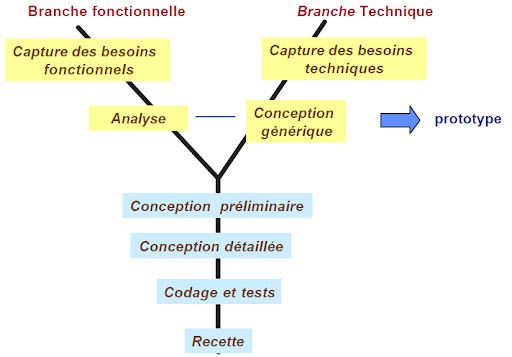
\includegraphics[width=0.75\textwidth,height=0.65\textwidth]{images/chapitre-1/2tup.png}
    \caption{Représentation de la méthodologie 2TUP \cite{2tup}}
    \label{fig:2tup-image}    
\end{figure}

\noindent Le processus s'articule ensuite autour de trois phases essentielles comme l'indique la Figure \ref{fig:2tup-image} :
\begin{itemize}[itemsep=2pt, parsep=2pt]
    \item \textbf{Une branche fonctionnelle} : Elle capitalise la connaissance du métier de l’entreprise. Cette branche capture des besoins fonctionnels, ce qui produit un modèle focalisé sur le métier des utilisateurs finaux.
    \item \textbf{Une branche technique} : Cette phase consiste à concevoir l'architecture du système, à définir les composants et à établir les spécifications techniques.
    \item \textbf{Une phase de réalisation} : Cette phase consiste à développer le système, à tester les composants et à valider le système.
\end{itemize}

\subsection{Raison du choix de la méthode 2TUP}
La méthode 2TUP offre une transparence en définissant un langage commun entre les membres de l'équipe, une inspection en fournissant une planification détaillée à court terme et une planification globale à long terme du projet, ainsi qu'une adaptation des exigences du projet selon les besoins de notre organisation et les circonstances imprévues.

\section{Planification avec le diagramme de Gantt}
Le diagramme de Gantt est un outil essentiel pour la gestion de projet. Il permet de planifier et de suivre les différentes étapes du projet au fil du temps. Notre projet, débuté le 5 Février et s’est déroulé durant 16 semaines, est représenté à travers ce diagramme. Les étapes clés incluent l'étude de préalable, l'analyse et la spécification des besoins, la conception, l'implémentation, les tests, ainsi que la rédaction du rapport. Chaque étape est visualisée dans le diagramme, fournissant une vue d'ensemble claire de la progression du projet au cours de la période de stage.
\begin{figure}[H]
    \centering
    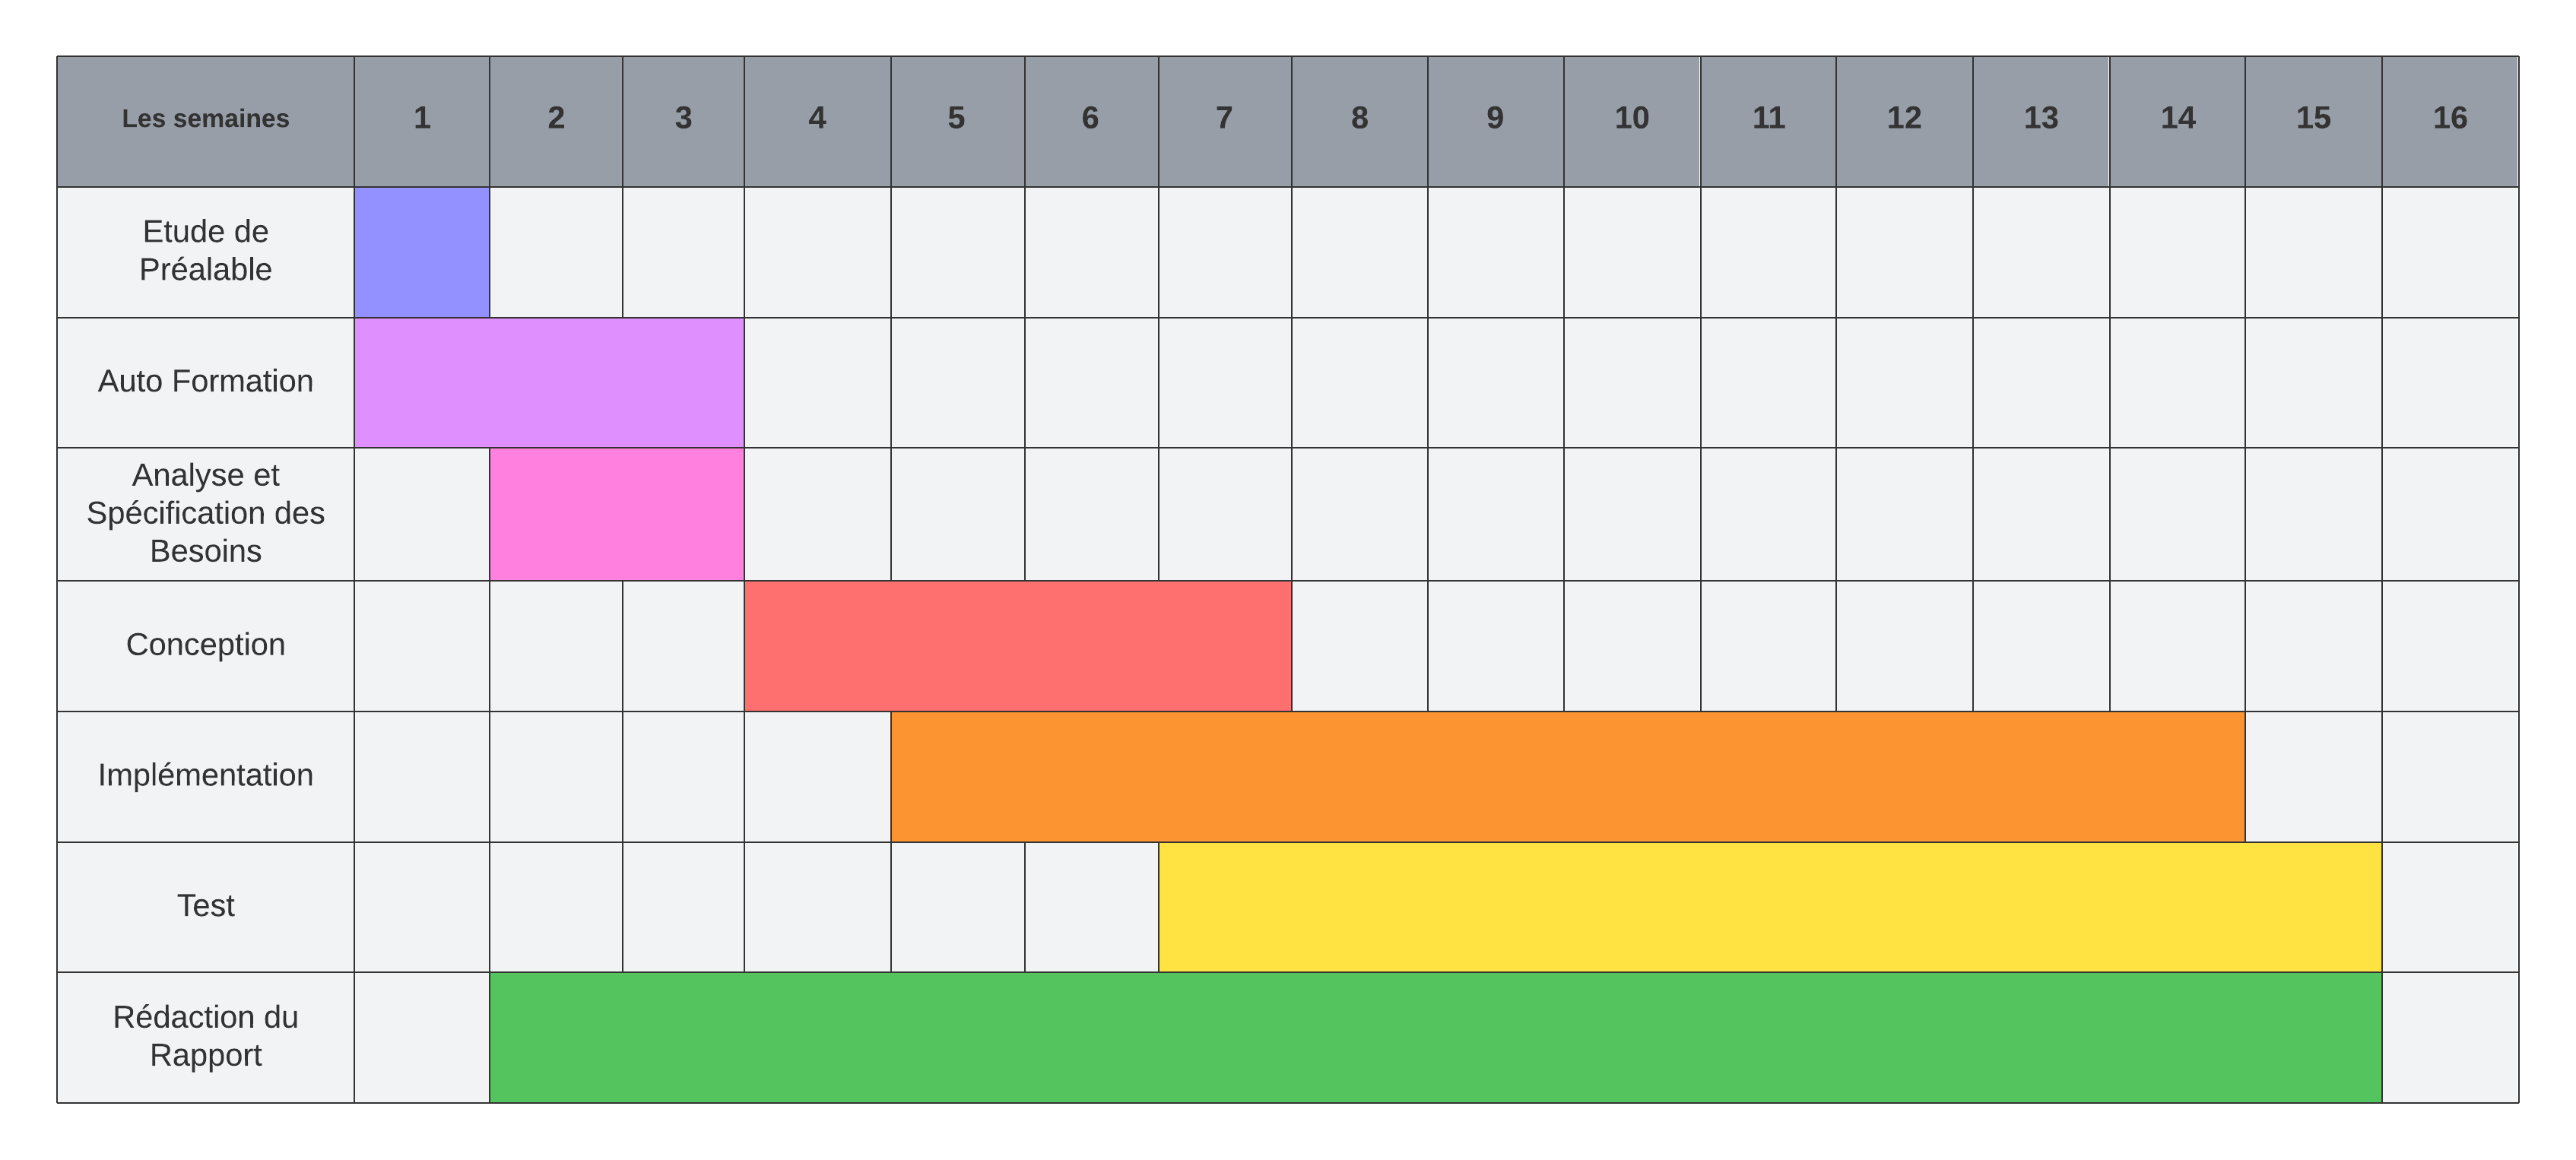
\includegraphics[width=1.1\textwidth,height=0.55\textwidth]{images/chapitre-1/gant.png}
    \caption{Diagramme de Gantt}
    \label{fig:gantt-diagram}    
\end{figure}

\section*{Conclusion}
Dans ce chapitre, nous avons défini le contexte général de notre projet. Ensuite, nous avons présenté les solutions existantes et leurs critiques pour définir les objectifs de notre projet et proposer une solution plus raffinée. Enfin, nous avons exposé notre choix méthodologique. Dans le chapitre suivant nous présenterons les fondements théoriques de notre projet, notamment, le cloud computing et l’intelligence artificielle.
